\section{Function Extraction}
Each function definition seen in the code is first collected. We start by
extracting invariants as well as pre- and post- conditions explicitly stated in
the code. We illustrate how Scala allows to express them in
Figure~\ref{fig:fe:example1}.

\begin{figure}[h]
    \centering
\begin{lstlisting}
class A (val next: A) {
  def test(a: A, b: A) = {
    require(a ne b) // pre-condition

    var c = a
    while(c ne b) {
        assert(c ne null) // invariant
        c = c.next
    }
    c

  } ensuring( r => r eq b ) // post-condition
}
\end{lstlisting}
    \caption{Expressing invariants and pre-/post-conditions in Scala}
    \label{fig:fe:example1}
\end{figure}

\section{CFG Generation}
For each function definintion extracted previously, we then generate the
corresponding control flow graph by converting complex statements into simple
assignments. We define the set of simple assignments in
Figure~\ref{fig:cfg:statements}.

\FloatBarrier
\begin{figure}[h]
    \centering

    \begin{tabular}{ l | l }
        CFG Statement               & Code example \\
        \hline
        AssignCast       & \verb/r = v.asInstanceOf[T]/  \\
        AssignTypeCheck  & \verb/r = v.isInstanceOf[T]/  \\
        AssignVal        & \verb/r = v/  \\
        AssignFieldRead  & \verb/r = obj.f/  \\
        AssignFieldWrite & \verb/obj.f = v/  \\
        AssignNew        & \verb/r = new T/  \\
        AssignApplyMeth  & \verb/r = obj.meth(..args..)/  \\
        AssignEQ         & \verb/r = v1 eq v2/  \\
        AssignNE         & \verb/r = v1 ne v2/  \\
    \end{tabular}

    \caption{CFG Statements}
    \label{fig:cfg:statements}
\end{figure}

It is worth noting that Scala converts most operations to method calls, and
introduces implicit getters and setters for non-private fields. For example,
the expression 
\begin{lstlisting}
val a = 2 * this.f
\end{lstlisting}
will be translated by the compiler into 
\begin{lstlisting}
val a = 2.*(this.f())
\end{lstlisting}
where \verb/*/ is a method on the class Int, and \verb/f/ is the implicit
getter method. We will then translate it into a simpler form analogous to
\emph{three-address code}:
\begin{lstlisting}
val tmp1 = this.f()
val tmp2 = 2.*(tmp1)
val a = tmp2
\end{lstlisting}

To illustrate the CFG generation phase, we provide in
Figure~\ref{fig:cfg:example1} the graph for the method defined in
Figure~\ref{fig:fe:example1} without its pre- or post-conditions.

\begin{figure}[h]
    \centering

    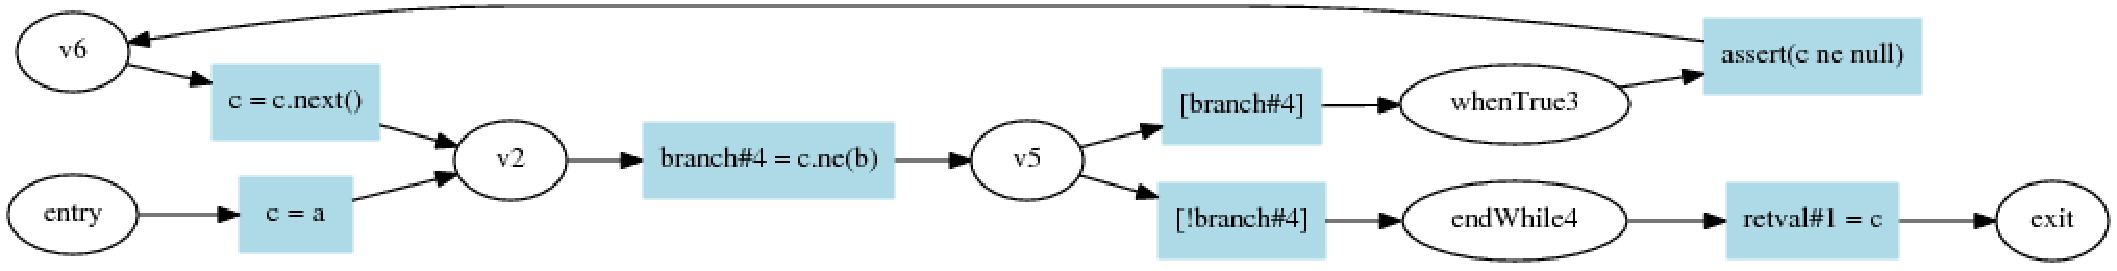
\includegraphics[scale=0.40]{images/cfg_example1}

    \caption{CFG Representation}
    \label{fig:cfg:example1}
\end{figure}

\section{Class Hierarchy}
This phase is responsible to build the complete graph representing the class
hierarchy. It will then be able to provide information such as $subtypes(C) :=
\{ T ~|~ T,C \in Classes \land T \subtypeeq C \}$, which is required by later
phases.

It is worth noting that in object oriented languages such as Scala,
$subtypes()$ is generally not bounded. This is caused by the fact that most
classes are not defined as \emph{final}, so that users can extend and redefine
parts of them. Scala also defines the concept of \emph{sealed} class, forcing
all \emph{direct} subtypes to be defined in the same source file. This property
is not sufficient in our case, since it only affects direct children (children
of non-sealed parents can be defined anywhere). In other words, the
\emph{sealed} property is not transitive.

In order to provide a useful analysis, we assume whole-code analysis: we
consider that classes analyzed represent the entire program, which allows us to
have bounded $subtypes()$ sets.  We argue that it is a reasonable and pragmatic
assumption, as it wouldn't be useful to analyze classes while assuming that
most methods could be in fact completely rewritten in imaginary sub-classes.
